% Formatting draft for JIRS; NOT SUBMITTED. Author fields intentionally blank.
% The official sn-jnl.cls is unchanged. No custom fonts. One manuscript TeX.
\documentclass[pdflatex,sn-mathphys-num]{sn-jnl}
\usepackage{graphicx,amsmath,amssymb,booktabs,array,textcomp}
\hypersetup{colorlinks=true,linkcolor=black,citecolor=black,urlcolor=blue,pdfauthor={}}
\setlength{\emergencystretch}{3em}
\newlength{\JournalTableWidth}
\providecommand{\tightlist}{\setlength{\itemsep}{0pt}\setlength{\parskip}{0pt}}
\providecommand{\passthrough}[1]{#1}
\providecommand{\pandocbounded}[1]{#1}
\raggedbottom
\begin{document}
\title{Category Priors and Geometric Feedback for Budget-Constrained Active Observation of Facilities}
% Author name, affiliation, email and ORCID: deliberately not supplied.
% \author*[1]{\fnm{} \sur{}}\email{}
% \affil*[1]{\orgdiv{},\orgname{},\orgaddress{\city{},\country{}}}
\abstract{Robots operating in reconfigured industrial workspaces must recover both spatial coverage and equipment surface geometry under limited observation budgets. This paper presents a category-conditioned active observation method for selecting useful viewing directions before geometry resolves a facility's configuration. The method combines category priors, bounded geometric feedback, diagnostic lookahead, and return-constrained planning in a hierarchical decision--execution loop. A finite-state planner evaluates observation sequences using public configuration templates, while measured depth alone contributes to volumetric reconstruction. We analyze when category information can reduce the cost of geometric diagnosis and demonstrate how contrary measurements correct an initially misleading prior. CPU simulations compare matched geometric and category-conditioned planners using identical sensing, reconstruction, and action budgets. On two reference layouts, category conditioning improves mean coverage--surface quality by 6.16\% at unchanged planar coverage. With the policy fixed, two additional background layouts yield a 2.98\% mean improvement, concentrated in a condition where the category cue changes the selected observation direction. An incorrect-prior comparison gives a 2.62\% gain for the complete correction policy. Budget and geometry variations show positive mean gains at the intermediate budget and a small reversal at the larger budget. Recorded trajectories and reconstructed surfaces support budget-sensitive benefits of early category information for facility observation.}
\keywords{active observation, facility documentation, category priors, geometric feedback, budget-constrained reconstruction}
\maketitle
\noindent\textbf{Categories:} (2), (5), (8).\quad\textit{Formatting draft; not submitted.}

\hypertarget{introduction}{%
\section{Introduction}\label{introduction}}

Industrial embodied systems depend on current environmental representations \cite{ref9}. Equipment rearrangement, workstation changes, and material relocation can invalidate a previously useful map. A robot may then need to reacquire the accessible layout and document nearby equipment. We consider a static environment during each acquisition task; changes occur between tasks, and dynamic obstacle avoidance is outside the scope.

Active mapping selects motion to improve an environmental model \cite{ref10}. For facility documentation, two objectives interact: observing the surrounding space and obtaining sufficient views of equipment surfaces. A robot can traverse a corridor and observe most of its accessible area while missing a recessed face or a structure on the far side of a cabinet. Additional travel through already visible open space may contribute little to that missing geometry. Under a finite action budget, the observation side and the timing of a turn can therefore matter as much as the distance traveled.

Categories may provide useful information before geometric disambiguation. If a recognized category is associated with an opening or service-side configuration, it can favor an observation route while the initial depth measurements remain ambiguous. This advantage is not automatic. An active geometric planner can also purchase a diagnostic view, revisit a location, and redirect its route. An incorrect category cue can waste the remaining budget unless contrary measurements change the belief and action. A meaningful semantic comparison must therefore retain active geometric planning in the control.

We ask whether a category cue can reduce the cost of selecting a useful observation direction under common navigation, reconstruction, and planning resources. This study makes three contributions:

\begin{enumerate}
\def\labelenumi{\arabic{enumi}.}
\tightlist
\item
  A category-conditioned observation method connects configuration priors, diagnostic lookahead, return constraints, and measured reconstruction in a planning--execution loop. A matched geometric control retains the same diagnosis, revisiting, and reconstruction capabilities, isolating the additional category information.
\item
  A two-configuration decision analysis relates category confidence, diagnostic cost, and directional utility. Recorded decisions and belief timelines explain how category cues select an early direction and how measured geometry corrects misleading priors.
\item
  Paired trajectories, actual TSDF meshes, fixed reconstruction checkpoints, and budget/geometry variations connect decision changes to measured surface recovery and identify the conditions under which category benefits persist or disappear.
\end{enumerate}

The study focuses on category-informed observation allocation for facility documentation. Its central question is when an early category cue changes a useful viewing decision, and how that decision survives correction by acquired geometry. Bayesian estimation and informative planning provide the foundations; the contribution lies in their task-specific integration and the connection between recorded decisions and measured reconstruction.

\hypertarget{related-work}{%
\section{Related Work}\label{related-work}}

\hypertarget{active-mapping-and-hierarchical-exploration}{%
\subsection{Active mapping and hierarchical exploration}\label{active-mapping-and-hierarchical-exploration}}

Active mapping couples motion selection with map quality and state estimation \cite{ref10}. TARE coordinates local and global exploration through representations at different resolutions \cite{ref5}. Learned hierarchical exploration, including Active Neural SLAM \cite{ref1}, also separates strategic decisions from execution. The present method uses this general separation for budgeted facility observation. Exact poses and a common safe graph allow the experiments to isolate the observation-planning contribution.

\hypertarget{reconstruction-driven-view-planning}{%
\subsection{Reconstruction-driven view planning}\label{reconstruction-driven-view-planning}}

Next-best-view methods select observations to improve reconstruction. GenNBV learns a policy using geometric, semantic, and action representations in a five-dimensional viewpoint space \cite{ref6}. Our implementation instead uses a finite public configuration family and discrete ground motion. Both internal policies can seek informative geometry. Their reconstruction backend uses Open3D \cite{ref4} and volumetric range integration \cite{ref11}, with measured depth as the sole source of surfaces. This separates using a prior to decide where to look from using it to complete an unobserved surface.

\hypertarget{semantic-information-for-observation-planning}{%
\subsection{Semantic information for observation planning}\label{semantic-information-for-observation-planning}}

Semantic inspection connects target meaning with observation requirements. SWAP combines exploration, semantic completion, and surface inspection \cite{ref2}, while semantics-aware predictive inspection planning uses repeated structures in semantic scene graphs to anticipate unseen inspection targets \cite{ref7}. VISTA combines task relevance and directional coverage in online semantic Gaussian mapping \cite{ref3}, and ActiveSGM couples semantic and geometric uncertainty when predicting observation informativeness \cite{ref8}. These works motivate information-aware allocation; semantic revisiting and structural prediction are not claimed as new concepts here.

These methods connect semantics to target requirements, repeated structures, query relevance, or uncertainty. Here, the category variable conditions an explicit hypothesis about a facility's hidden configuration. We examine when this prior changes the choice between return-feasible observation routes and how acquired geometry revises that choice. Belief-based decisions and informative path planning supply established foundations \cite{ref12,ref13}. SWAP-I/VISTA-I comparisons adapt selected mechanisms to common candidates and fusion; native TARE integration provides engineering evidence. The primary category contrast uses matched internal planners, while the adapted comparisons do not represent complete-system state-of-the-art rankings.

\hypertarget{problem-formulation}{%
\section{Problem Formulation}\label{problem-formulation}}

The local task contains one facility with an unknown configuration \(h\in\{0,1\}\). Both policies receive two public templates, a facility coordinate frame, an initial pose \(s_0\), and a safe pose graph. They receive RGB-D, planar scan, and pose observations only when those observations are acquired. The category--configuration association is manually specified public knowledge. Evaluation references, true configuration identifiers, and actual measurements from unexecuted actions are unavailable to the planner.

A forward motion of 1 m or a 90\ensuremath{^{\circ}} turn consumes one action and acquires a sensor frame. An identical 18-action observation prefix precedes autonomous selection within total budget \(B\). The original confirmation uses \(B=42\); the extension also evaluates 30 and 54. A qualified task must remain collision-free, finish within budget, attain at least 80\% planar coverage, and return to the initial position and orientation. The experiment consequently tests allocation after common observation, rather than unknown-environment exploration from the first action.

The principal measured score combines planar coverage and surface quality:

\[
C_{\rm map}=\frac{|\{c\in\mathcal R:m_T(c)\ne-1\}|}{|\mathcal R|},
\qquad F_{1,\tau}=\frac{2P_\tau R_\tau}{P_\tau+R_\tau},
\qquad J_5=C_{\rm map}F_{1,0.05}.
\]

Here \(\mathcal R\) is the start-reachable evaluation grid, \(m_T\) is the terminal measured occupancy map, and \(-1\) denotes an unobserved cell. \(P_\tau\) and \(R_\tau\) denote surface precision and recall within distance \(\tau\), measured in meters. Section 5.1 specifies the evaluation region, sampling, and qualification rules.

The desired policy maximizes expected measured \(J_5\) using acquired information while respecting budget and return constraints. Online template exposure is only its planning surrogate. A larger predicted opportunity need not produce a more accurate fused mesh, and additional observations do not guarantee improvement at every surface threshold.

\hypertarget{observation-planning-with-correctable-category-priors}{%
\section{Observation Planning with Correctable Category Priors}\label{observation-planning-with-correctable-category-priors}}

\hypertarget{system-overview-and-planning-state}{%
\subsection{System overview and planning state}\label{system-overview-and-planning-state}}

The method couples a decision layer with an execution layer: the former selects an observation subgoal, and the latter checks its legality and return cost before acquiring another measurement. In the local implementation, each subgoal is one atomic action. Four interfaces connect perception, planning, and feedback (Table 1 and Figure 1). Their names specify responsibilities in the CPU implementation; they do not denote four independently trained networks. The category-conditioned policy S and geometric control G share the graph, public templates, planner, and reconstruction backend. G retains diagnostic views and revisiting.

\begin{table}[!htbp]
\caption{Four CPU interfaces and their executed roles}\label{tab:1}
\small\setlength{\tabcolsep}{3pt}
\setlength{\JournalTableWidth}{\dimexpr\linewidth-4\tabcolsep\relax}
\begin{tabular}{@{}>{\raggedright\arraybackslash}p{0.16\JournalTableWidth} >{\raggedright\arraybackslash}p{0.32\JournalTableWidth} >{\raggedright\arraybackslash}p{0.52\JournalTableWidth}@{}}
\toprule
Interface & Input & Output and role \\
\midrule
OV-SDF & Acquired RGB, pose, measured-map summary & Register category support and configuration prior \\
STGHP & Graph, exposure sets, beliefs, remaining budget & Compare feasible continuations and select a subgoal \\
RPN-UQ & Proposed edge, budget, return distance & Permit or reject the executable action \\
IGCR & Acquired depth/scan and public predictions & Bound geometric evidence and revise belief \\
\bottomrule
\end{tabular}
\end{table}

\begin{figure}[!htbp]
\centering
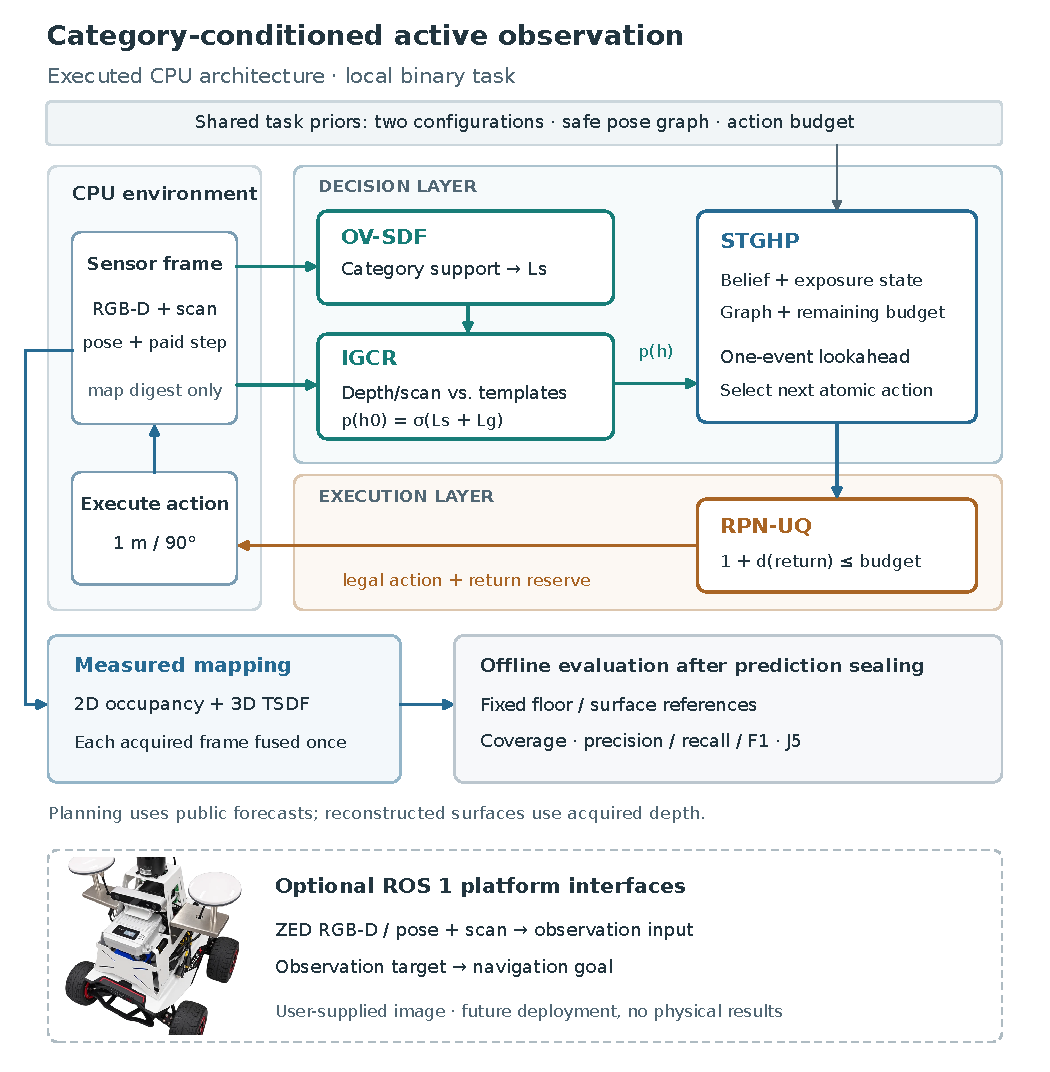
\includegraphics[width=\linewidth,height=.67\textheight,keepaspectratio]{Fig1.pdf}
\caption{CPU observation and execution architecture. Category and geometric evidence update the belief used for planning; acquired depth separately enters TSDF fusion. The unchanged user-supplied robot image illustrates prospective ROS 1 interfaces. All reported performance is simulated; the diagram uses programmatically drawn vector elements}\label{fig:1}
\end{figure}

After action \(t\), the planning state is

\[
x_t=(s_t,b_t,M_{0,t},M_{1,t},p_t,\mathcal V_t),\qquad b_t=B-t.
\]

Here \(s_t\) includes position and heading, \(p_t\) weights configuration 0, and \(\mathcal V_t\) contains measured poses. Each \(M_{h,t}\) records the union of floor samples and surface patches predicted visible from previously observed poses under public template \(h\). These exposure sets support prospective planning; the measured map separately integrates acquired depth. Neither hidden configuration identifiers nor evaluation surfaces enter the state. The common 18-action prefix updates observations and returns to \(s_0\); subsequent actions depend on the resulting belief.

Both hypotheses remain available throughout execution. Category information changes their weights rather than selecting a template as reconstructed truth. The online belief module additionally retains geometric log-support and category-registration history, while each planning call receives their current combined weight. This separates two questions: which configuration the acquired evidence supports, and which affordable observation sequence is valuable under that uncertainty.

\hypertarget{category-support-and-geometric-correction}{%
\subsection{Category support and geometric correction}\label{category-support-and-geometric-correction}}

OV-SDF registers a category when its marker occupies at least 16 exact-color pixels at each of two distinct XY positions, without a competing marker in those frames. Registration supplies \(L_t^s=\pm\log9\); repeated detections do not multiply this prior, and conflicting category support clears it. G uses \(L_t^s=0\). Synthetic markers provide a controlled category channel, independently of natural-image recognition performance.

IGCR compares acquired depth and scan measurements with both public predictions. Let \(e_{h,t}^{k}\) be the mean residual loss for eligible modality \(k\) under template \(h\), and \(\mathcal K_t\) its valid-modality set. At a newly visited pose,

\[
\begin{aligned}
\delta_t=\operatorname{clip}_{[-6,6]}
\left(\frac{1}{|\mathcal K_t|}\sum_{k\in\mathcal K_t}
\bigl(e_{1,t}^{k}-e_{0,t}^{k}\bigr)\right),\\
L_t^g=\operatorname{clip}_{[-24,24]}(L_{t-1}^g+\delta_t),\qquad
p_t=\sigma(L_t^g+L_t^s).
\end{aligned}
\]

Here \(\sigma(z)=(1+e^{-z})^{-1}\). The increment is zero when no modality qualifies or the pose has already supplied evidence. Residuals use samples where public predictions differ by more than \(10^{-5}\) m. Depth requires eight valid pixels and normalized disparity residual \((57.6/z-57.6/\widehat z_h)/0.25\); scan requires three valid beams and residual \((r-\widehat r_h)/0.02\). Each sample contributes half its squared residual, capped at 12.5. Missing measured returns are ignored; a missing predicted depth return receives the capped loss. Eligible modality means receive equal weight.

These bounded pseudo-likelihoods prevent individual extreme residuals from dominating. They are not calibrated probabilities, and excluding exact repeats does not establish independence between neighboring views. New depth from a repeated pose still contributes to fusion. An incorrect prior remains correctable: for \(L^s>0\), configuration-1 support reaches \(\eta>1/2\) whenever

\[
L_t^g\le-L^s-\operatorname{logit}(\eta).
\]

This threshold is attainable only if sufficient contrary observations occur and the cumulative cap permits it. The finite prior therefore expresses a revisable preference rather than a permanent semantic constraint.

\hypertarget{predictive-value-and-diagnostic-lookahead}{%
\subsection{Predictive value and diagnostic lookahead}\label{predictive-value-and-diagnostic-lookahead}}

For template \(h\), let \(\mathcal F_h\) contain its floor samples, \(\mathcal P_h\) its exterior vertical patches, \(a_u\) the patch area, and \(A_h\) the total exterior vertical area. Writing \(M_h^f\) and \(M_h^s\) for the corresponding exposed subsets gives

\[
\widetilde C_h=\frac{|M_h^f|}{|\mathcal F_h|},\qquad
\widetilde S_h=\min\left(1,\frac{\sum_{u\in M_h^s}a_u}{A_h}\right),\qquad
\widetilde J_h=\widetilde C_h\widetilde S_h.
\]

Thus \(\widetilde S_h\) is an exposed-area fraction, not reconstructed surface F1. The surrogate rewards opportunities to observe missing surfaces but does not model TSDF error or improvements from repeated measurements. Its relation to measured \(J_5\) is tested empirically.

Exposure is accumulated by set union, so viewing an already exposed patch supplies no additional proxy area. Changing direction can still reveal previously occluded patches. Floor samples are those declared by the public planning model, distinct from the finer reachable-cell grid used to measure \(C_{\rm map}\). Consequently, neither component of the surrogate is substituted for an endpoint measurement. Keeping both representations makes the planning assumption explicit: access to additional surface area is a useful, imperfect predictor of reconstructed quality.

Let \(M=(M_0,M_1)\). Stopping requires the complete initial pose and adequate predicted floor exposure under both configurations:

\[
Z(s,M,p)=
\begin{cases}
p\widetilde J_0(M_0)+(1-p)\widetilde J_1(M_1),
&s=s_0,\ \min_h\widetilde C_h(M_h)\ge0.8,\\
-\infty,&\text{otherwise}.
\end{cases}
\]

STGHP approximates belief-space planning \cite{ref12,ref13} with one future diagnostic event per planning call. Diagnostic candidates are determined from public sensor predictions: treating each template prediction as a hypothetical observation must yield geometric evidence at least \(+\log99\) for configuration 0 and at most \(-\log99\) for configuration 1. Previously measured poses are excluded. This identifies potentially discriminative viewpoints without obtaining their actual observations.

For an anticipated diagnosis of assumed accuracy \(r_d=0.99\), the branch weights and updated planning beliefs are

\[
\begin{aligned}
\lambda_0&=pr_d+(1-p)(1-r_d),\qquad \lambda_1=1-\lambda_0,\\
p^{(0)}&=\frac{pr_d}{\lambda_0},\qquad
p^{(1)}=\frac{p(1-r_d)}{\lambda_1}.
\end{aligned}
\]

Let \(q\in\{0,1\}\) indicate whether this event remains available. Action \(a\) reaches \(s'\), consumes one action, and updates \(M'_h=M_h\cup E_h(s')\), where \(E_h\) is public predicted exposure. The continuation and value recursions are

\[
Q_q(a)=
\begin{cases}
\sum_{y=0}^{1}\lambda_y V_0(s',b-1,M',p^{(y)}),
&q=1,\ s'\text{ diagnostic},\\
V_q(s',b-1,M',p),&\text{otherwise},
\end{cases}
\] \[
V_q(s,b,M,p)=\max\left\{Z(s,M,p),\max_{a\in\mathcal A(s)}Q_q(a)\right\}.
\]

At \(b=0\), only stopping is available. States whose return distance exceeds \(b\) are infeasible, as are diagnostic actions with either infeasible branch. Forecast beliefs remain inside the current calculation. The controller executes only the first selected action, updates belief from acquired measurements, and replans. The category strength 0.9 and forecast accuracy 0.99 are fixed design settings shared across the comparisons, rather than measured classifier or sensor accuracies.

The recursion evaluates complete remaining continuations, rather than immediately visible area alone. Anticipated diagnosis is useful only through the different actions it may enable afterward. Requiring a feasible continuation in both branches prevents a low-weight configuration from being silently discarded to satisfy the return and coverage gates. The approximation limits the number of belief changes within one forecast; it does not limit the number of measured corrections over the executed trajectory. A later call can anticipate another diagnostic event after assimilating the latest frame.

\hypertarget{budgeted-execution-and-reconstruction}{%
\subsection{Budgeted execution and reconstruction}\label{budgeted-execution-and-reconstruction}}

RPN-UQ accepts a legal edge only if

\[
1+d_{\rm return}(s')\le b_t,
\]

where return distance includes restoration of the starting heading. On the fixed graph with unit action costs, this preserves an affordable return path: after each accepted action, \(d_{\rm return}(s_{t+1})\le b_t-1=b_{t+1}\). This certificate concerns graph feasibility; task qualification additionally requires measured coverage, collision-free execution, and actual return.

\par\medskip\noindent\begin{minipage}{\linewidth}
\small\hrule\vspace{0.6em}
\textbf{Algorithm 1. Category-conditioned receding-horizon observation.}

\begin{verbatim}
Input: common graph, templates, budget B, prefix, policy G or S
Initialize belief support, exposures, and visited poses
Repeat:
  Read the initial frame or latest executed-action frame
  Fuse acquired depth exactly once into the measured TSDF
  OV-SDF: register category; IGCR: update geometric evidence
  Add current template exposures and record the measured pose
  If collision or budget exhaustion: record termination; exit
  If the shared prefix is unfinished: select its next action
  Otherwise:
    Exclude measured poses from diagnostic candidates
    STGHP: solve V1 from current state and remaining budget
    If infeasible or a resource cap is exceeded: fail; exit
    If stopping is optimal within tolerance: stop; exit
    Select the first maximizing action in fixed graph-edge order
  RPN-UQ: check legality and the return-budget inequality
  If rejected: record the termination reason; exit
  Execute one action, charge its cost, and obtain the next frame
Output: measured map, trajectory, observations, and stop reason
\end{verbatim}
\vspace{0.4em}\hrule
\end{minipage}\par\medskip


Equal-valued choices use a \(10^{-12}\) tolerance and fixed edge order. The shared Open3D CPU TSDF \cite{ref4,ref11} uses 4 cm voxels and 12 cm truncation; public templates never contribute synthetic depth. Outputs precede independent endpoint evaluation. Incorrect-prior controls exchange category interpretation; the no-correction variant additionally disables measured correction and forecast diagnosis.

For \(N\) poses and exposure bitset lengths \(m_0,m_1\), the cached state count is conservatively bounded by \(K\le3N(B+1)2^{m_0+m_1}\), covering the initial and two post-diagnosis weights. With maximum out-degree \(d\), bitset-update cost \(T_m\), and terminal-evaluation cost \(T_z\), planning costs \(O(K(dT_m+T_z))\), excluding return-distance preprocessing. Each call permits 1.5 million cached states and approximately 20 s; elapsed time is checked every 1024 new states and at selection completion. This finite implementation supports the controlled task, with exponential exposure-state dependence.

\hypertarget{decision-interpretation-and-conditions-for-benefit}{%
\subsection{Decision interpretation and conditions for benefit}\label{decision-interpretation-and-conditions-for-benefit}}

A recorded example connects the recursion to robot behavior. After the common prefix in P00, G assigns both configurations weight 0.5; left/right continuation values of 0.650944 tie. With configuration-1 category support 0.9, S obtains 0.668008/0.711865 and turns right at action 19. A misleading prior can subsequently reverse: geometric evidence of \(-6\) at step 28 gives configuration-1 weight \(1-\sigma(-6+\log9)=0.978178\), followed by a changed action at step 29. These are planning values and belief weights; measured reconstruction outcomes are reported separately.

The underlying tradeoff can be expressed using established belief-based decision principles \cite{ref12,ref13}. Assume two initially equally likely configurations, two return-feasible routes, matched utility \(U_+\), mismatched utility \(U_-\), and \(\Delta=U_+-U_->0\). A category cue has symmetric reliability \(r_c\ge1/2\). Optional geometric diagnosis has symmetric reliability \(r_d\ge1/2\), is conditionally independent given configuration, and costs utility \(\kappa\). Both routes remain feasible afterward. For current belief \(p\), direct choice succeeds with probability \(m=\max(p,1-p)\); optimal choice after diagnosis succeeds with probability \(\max(m,r_d)\). Its net value is

\[
\Delta\max(0,r_d-m)-\kappa.
\]

G benefits from diagnosis when \(\kappa<(r_d-1/2)\Delta\), whereas a category-conditioned decision requires \(\kappa<(r_d-r_c)_+\Delta\), with \(\kappa\ge0\). An informative cue can therefore avoid a diagnostic detour while preserving a useful observation direction. Its benefit disappears when geometry already resolves the choice or route utilities coincide. When \(r_d\ge r_c\) and diagnosis is free, both policies can attain the same expected directional utility; a free but less reliable diagnosis need not remove the category advantage. These analytical reliabilities are assumptions distinct from implementation settings. The argument identifies conditions for improved allocation; it does not guarantee better measured reconstruction under the exposure surrogate.

The practical consequence is a conditional experimental prediction: a category cue should matter when it changes a consequential route ranking before equivalent geometric evidence is affordable. If geometry and category already favor the same route, identical actions and quality are expected. Tests therefore examine action changes, acquired surfaces, and measured quality together, rather than interpreting stronger belief alone as a mapping improvement.

\hypertarget{experiments-and-results}{%
\section{Experiments and Results}\label{experiments-and-results}}

The experiments address four questions: whether category information improves surface recovery at matched coverage; whether acquired geometry corrects a misleading cue; how observation allocation compares with other planning mechanisms; and how the benefit changes with budget, geometry, and background layout.

\hypertarget{experimental-setup-and-matched-comparisons}{%
\subsection{Experimental setup and matched comparisons}\label{experimental-setup-and-matched-comparisons}}

The simulator supplies 96\ensuremath{\times}72 depth images over a 4 m range and a 360\ensuremath{^{\circ}} planar scan with 180 beams over 8 m. Poses are exact. Depth noise has a standard deviation of 0.25 pixels in reference disparity; no additional random scan noise is applied. The experiments isolate planning under controlled observations rather than reproduce physical sensor errors.

The evaluator derives the start-reachable safe-cell set \(\mathcal R\) using a 0.2 m grid and 0.2 m robot radius. It contains 588 cells in P00 and 668 in P01. A nonunknown cell counts as observed, including one marked occupied, so coverage is not occupancy-classification accuracy. Ground truth is used after prediction sealing, not to supply runtime measurements.

Surface precision and recall follow distance-threshold comparison \cite{ref14}. Precision queries the reference from sampled predicted surfaces; recall queries the prediction from fixed exterior vertical reference surfaces. The prediction is cropped to the common bounding box of both templates with a 0.20 m margin, and the known ground is removed. Thus, errors outside this region do not enter precision. No registration or hole filling is applied. Thresholds are fixed at 2, 5, and 10 cm, with 5 cm primary; empty predictions receive zero quality. Coverage, precision, recall, and task qualification accompany the product to avoid hiding its components.

Confirmation freezes the controller and uses a held-out noise seed on two previously seen parent layouts, each with two configurations: eight runs and four G/S pairs. Separate development comparisons use incorrect category interpretation X and Xnf, which also disables measured correction and future diagnostic anticipation. Their contrast evaluates the whole correction policy. Replays and alternative thresholds reuse these trajectories; they do not increase the number of independent layouts or trials. All controls retain active geometric reasoning.

The recorded software is Python 3.12.3, NumPy 1.26.4, SciPy 1.11.4, and Open3D 0.19.0, with one OpenMP, OpenBLAS, and MKL thread. No GPU is required. Figures use actual recorded actions and measured meshes except the explicitly schematic architecture diagram.

\begin{figure}[!htbp]
\centering
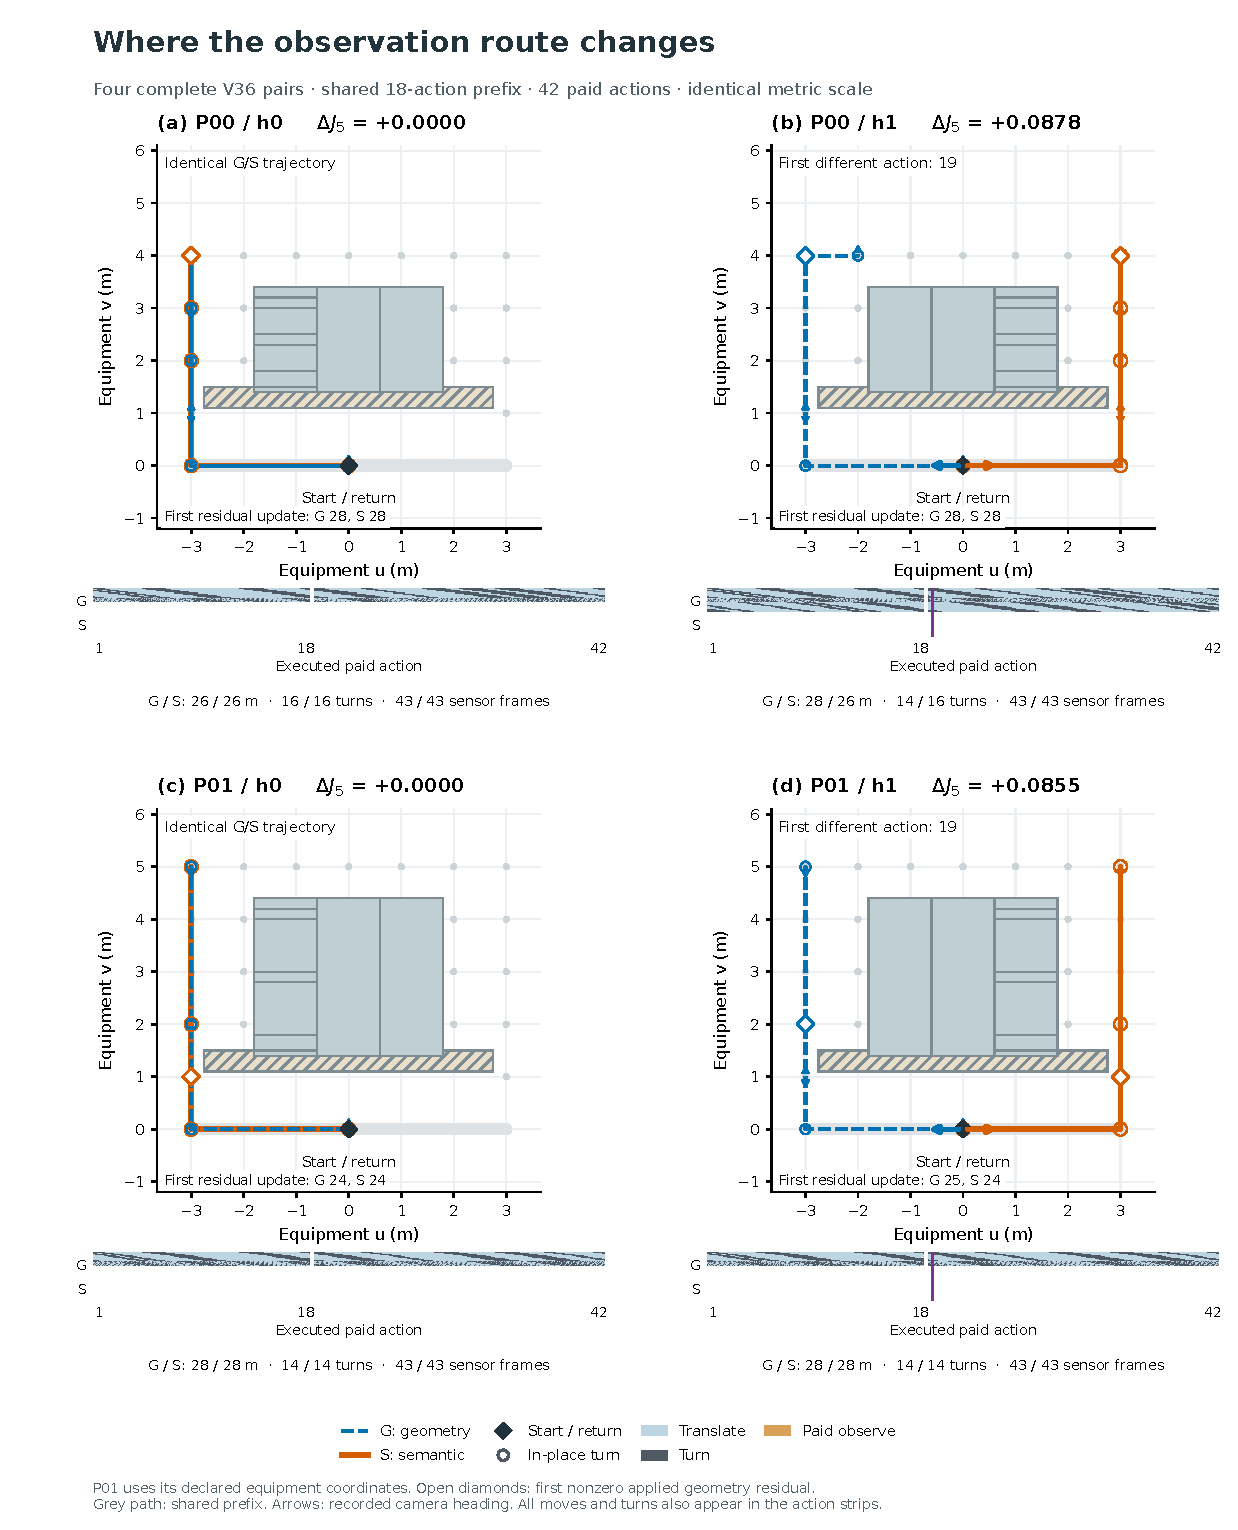
\includegraphics[width=\linewidth,height=.67\textheight,keepaspectratio]{Fig2.pdf}
\caption{Both configurations of P00 and P01, with common 18-action prefixes, saved paths, and complete action strips. Panels share metric scale. Circles denote turns, arrows recorded headings, and open diamonds first applied geometric feedback. The two h0 routes coincide; both h1 pairs diverge at action 19}\label{fig:2}
\end{figure}

\hypertarget{surface-reconstruction-at-matched-coverage}{%
\subsection{Surface reconstruction at matched coverage}\label{surface-reconstruction-at-matched-coverage}}

Across the four confirmation conditions in Table 2, mean \(J_5\) increases from 0.702576 to 0.745881, a relative improvement of \textbf{6.1638\%}. Every run uses 42 actions, avoids collision, and returns exactly. Mean coverage is identical at 0.952544; mean surface F1 increases from 0.737490 to 0.782951. This decomposition attributes the observed joint-score gain to surface reconstruction at matched planar coverage.

\begin{table}[!htbp]
\caption{Complete confirmation pairs; relative change compares policy means}\label{tab:2}
\small\setlength{\tabcolsep}{3pt}
\setlength{\JournalTableWidth}{\dimexpr\linewidth-6\tabcolsep\relax}
\begin{tabular}{@{}>{\raggedright\arraybackslash}p{0.32\JournalTableWidth} >{\raggedright\arraybackslash}p{0.22\JournalTableWidth} >{\raggedright\arraybackslash}p{0.22\JournalTableWidth} >{\raggedright\arraybackslash}p{0.24\JournalTableWidth}@{}}
\toprule
Layout/configuration & G: \(J_5\) & S: \(J_5\) & S\ensuremath{-}G \\
\midrule
P00/h0 & 0.772200 & 0.772200 & 0 \\
P00/h1 & 0.672703 & 0.760456 & +0.087753 \\
P01/h0 & 0.727281 & 0.727281 & 0 \\
P01/h1 & 0.638118 & 0.723586 & +0.085468 \\
Mean & 0.702576 & 0.745881 & +0.043305 \\
\bottomrule
\end{tabular}
\end{table}

In both h1 cases, category conditioning changes the first autonomous turn. The resulting surface recall rises from 0.5958 to 0.7249 in P00 and from 0.5555 to 0.6845 in P01. Both h0 pairs follow identical trajectories. The relative mean gains at 2 and 10 cm are 5.5040\% and 6.2110\%, respectively. These descriptive sensitivities do not establish statistical significance across unseen layouts.

\begin{figure}[!htbp]
\centering
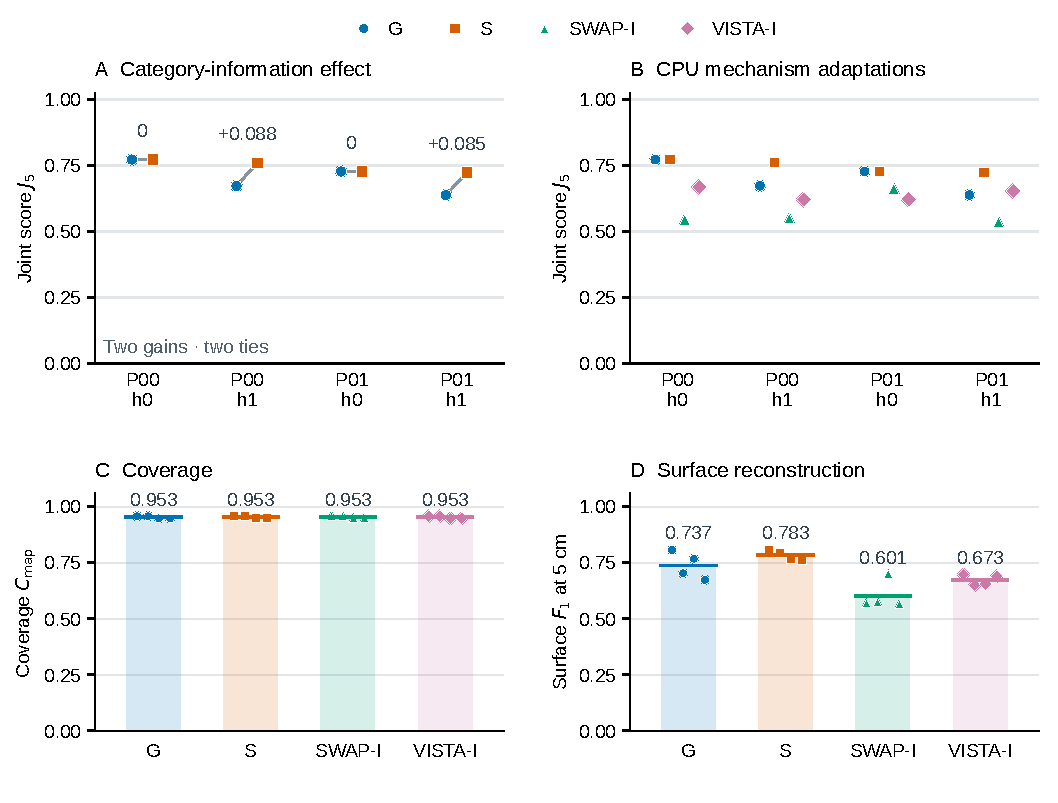
\includegraphics[width=\linewidth,height=.67\textheight,keepaspectratio]{Fig3.pdf}
\caption{Paired outcomes for all four conditions and the coverage/F1 decomposition. Points represent conditions; horizontal caps indicate means rather than confidence intervals. G/S trajectories reused in the external-mechanism panel are not additional evidence}\label{fig:3}
\end{figure}

Actual endpoint meshes in Figure 4 show the recovered side structures using matched cameras and scales. P00/h1 needs 28 m and 14 turns for G versus 26 m and 16 turns for S; P01/h1 uses 28 m and 14 turns for both. Every run acquires the same number of frames. The effect therefore depends on allocating observations differently, rather than increasing sensing or travel.

\begin{figure}[!htbp]
\centering
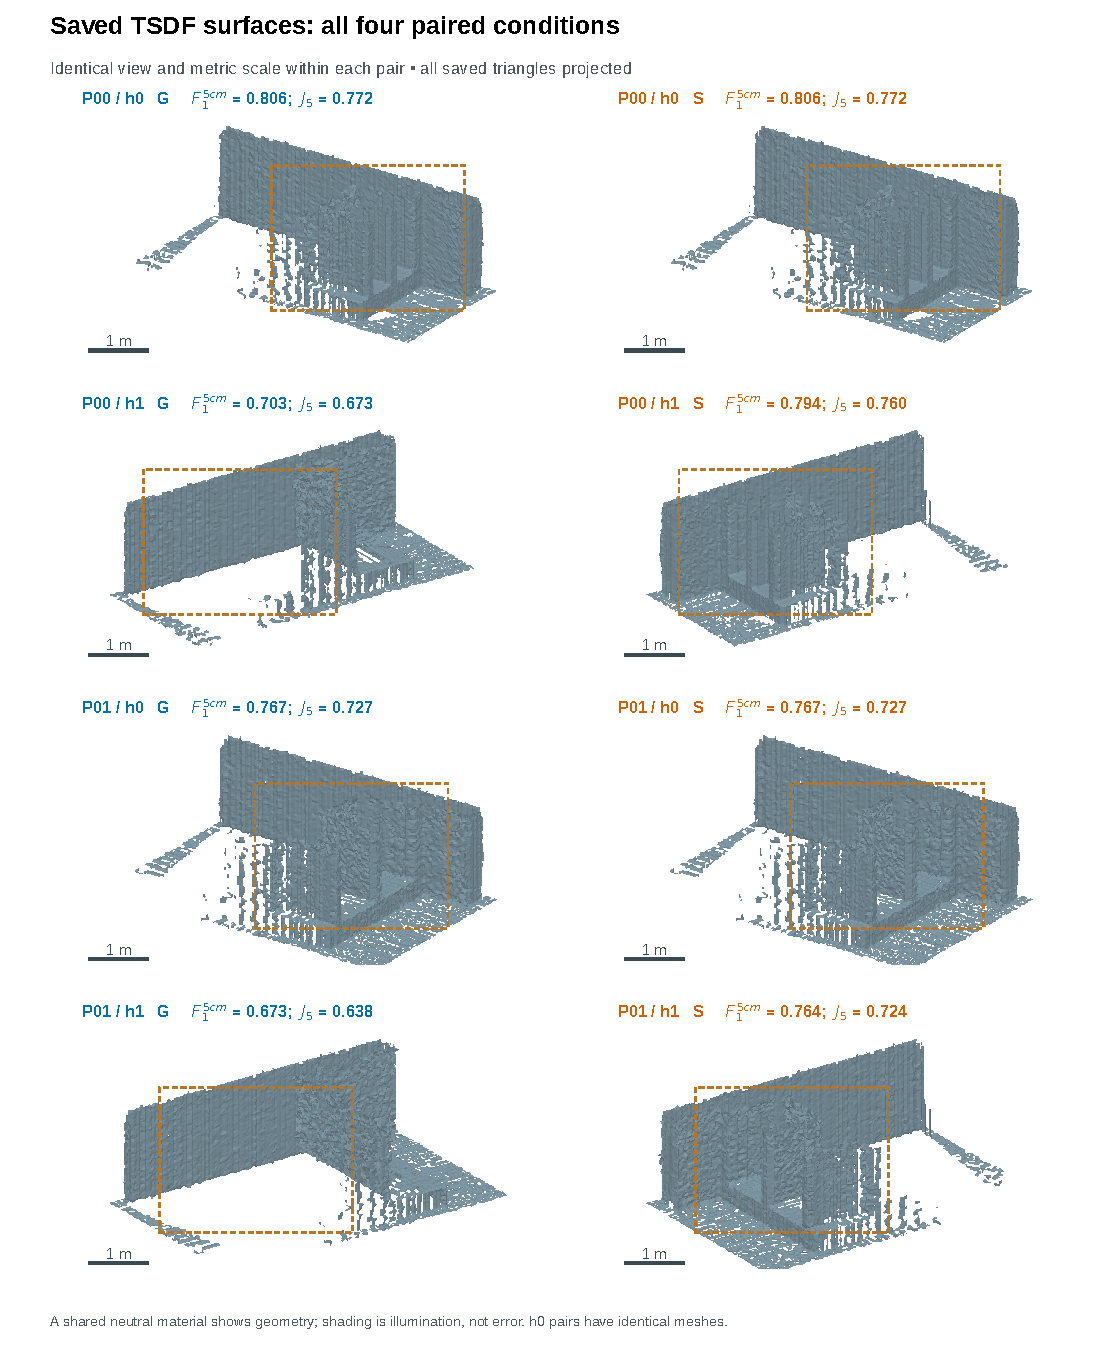
\includegraphics[width=\linewidth,height=.67\textheight,keepaspectratio]{Fig4.pdf}
\caption{Saved TSDF meshes in the common evaluation region. Each pair shares camera, scale, material, and lighting; all stored triangles are rendered. Both h0 pairs remain identical. Shading represents illumination, not error. Dashed windows correspond to matched detail views (Online Resource 1); no smoothing, template completion, or local quality score is introduced}\label{fig:4}
\end{figure}

\hypertarget{geometric-correction-and-reconstruction-progress}{%
\subsection{Geometric correction and reconstruction progress}\label{geometric-correction-and-reconstruction-progress}}

The P00 development timeline in Figure 5 connects the decision example in Section 4.5 to acquired evidence. Category support changes the first autonomous observation direction at action 19, while subsequent geometric measurements can reverse the influence of an incorrect cue.

With the incorrect cue, X initially assigns configuration 1 a weight of 0.1. At step 28, 1092 informative depth pixels provide sufficient contrary evidence to raise this weight to 0.978178. X then moves forward at action 29, while Xnf turns right. Across the two development configurations, X improves mean \(J_5\) over Xnf from 0.655065 to 0.672254, or 2.6241\%. Because Xnf also removes anticipated diagnosis, this is not an isolated posterior-update ablation. At the stricter 2 cm threshold, the h1 difference is \ensuremath{-}0.00216, indicating that correction does not improve every surface-scale measure.

\begin{figure}[!htbp]
\centering
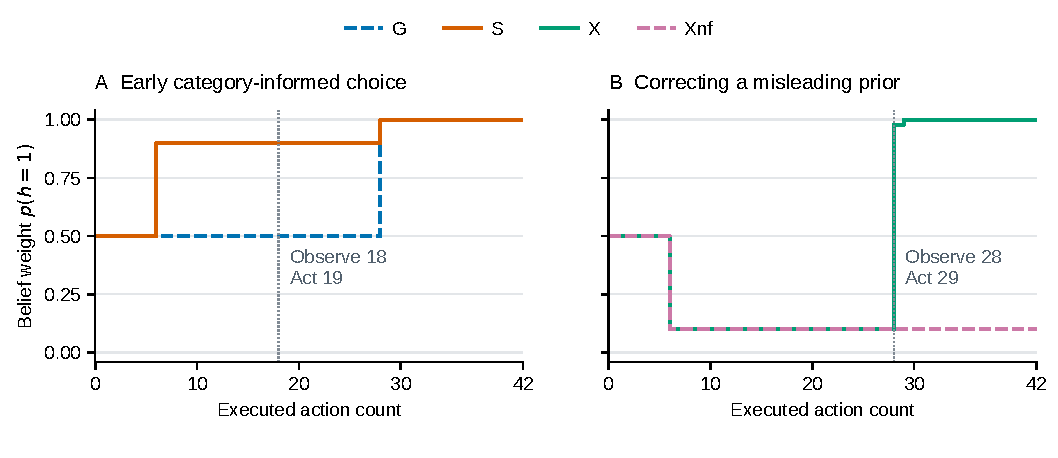
\includegraphics[width=\linewidth,height=.67\textheight,keepaspectratio]{Fig5.pdf}
\caption{Acquired category support changes action 19; contrary measured geometry at step 28 changes action 29. Curves are uncalibrated configuration weights from P00/h1 development logs. The timeline explains the decisions without adding counterfactual endpoint trials}\label{fig:5}
\end{figure}

We further reintegrate the eight saved confirmation trajectories at 18, 24, 30, 36, and 42 paid actions: \textbf{40 measured checkpoints}, with unchanged observations, poses, fusion settings, and evaluator. All 16 previously available prefix/endpoint checkpoints reproduce their original metrics exactly. Coverage matches within every pair at every checkpoint and reaches its endpoint value by action 30. Later differences mainly accompany increased surface recall and F1. P00/h1 is still slightly worse for S at action 24 (\ensuremath{-}0.000819), then positive at 30, 36, and 42; P01/h1 is already positive at 24. Both h0 pairs remain tied. Intermediate states may not satisfy return or coverage requirements and are not successful terminal trials.

\begin{figure}[!htbp]
\centering
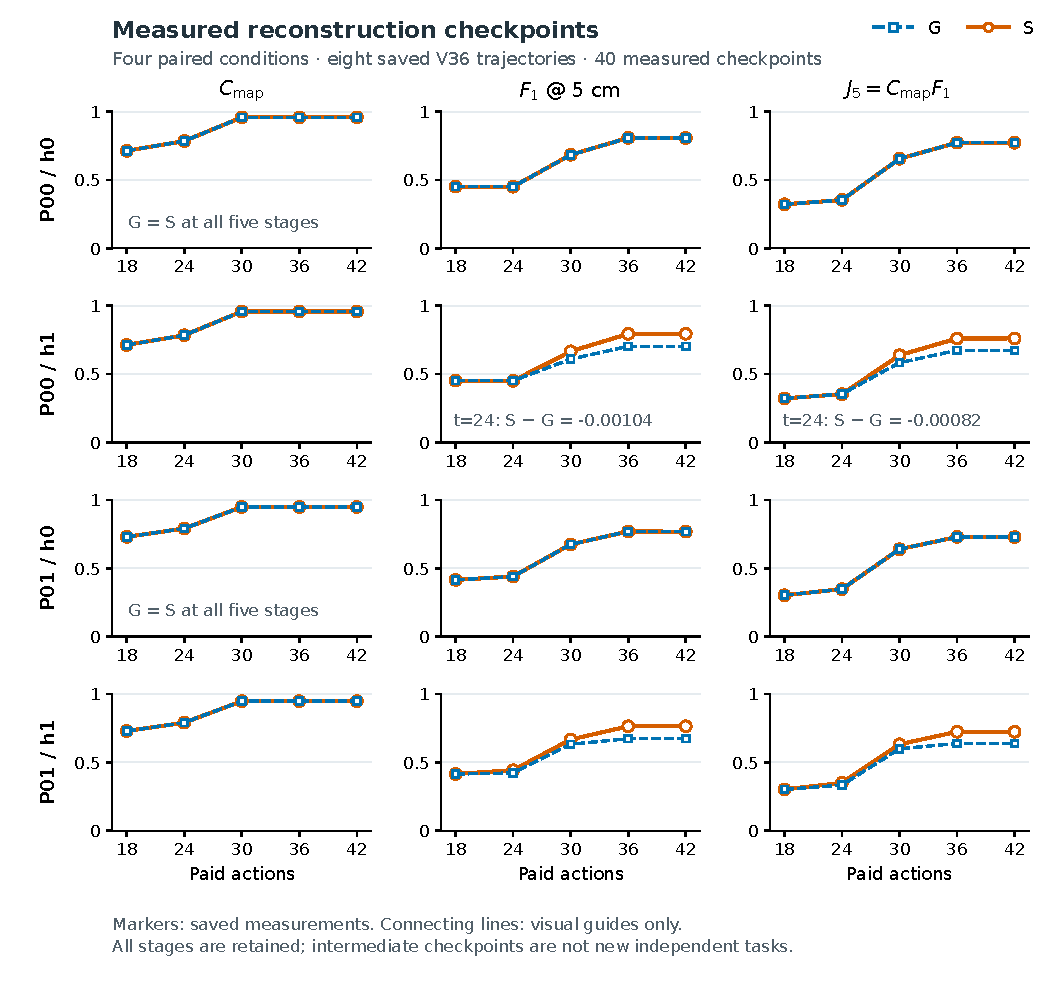
\includegraphics[width=\linewidth,height=.67\textheight,keepaspectratio]{Fig6.pdf}
\caption{Coverage, 5 cm surface F1, and joint quality for all four paired conditions at all five measured checkpoints. Markers are actual measurements; connecting lines are visual guides. Both h0 ties and the early P00/h1 negative difference remain visible, with common 0--1 axes. Forty checkpoints reuse eight trajectories and add no independent runs. Complete precision/recall figure (Online Resource 2) and actual stage meshes (Online Resource 3) accompany the data}\label{fig:6}
\end{figure}

\hypertarget{comparison-with-common-cpu-planning-mechanisms}{%
\subsection{Comparison with common-CPU planning mechanisms}\label{comparison-with-common-cpu-planning-mechanisms}}

SWAP-I and VISTA-I each complete four qualified tasks using common sensing and fusion. Table 3 summarizes their measured endpoints. Their lower scores indicate different observation allocation in this task, while changed objectives and planner details prevent attributing the full differences to category information. A native TARE node additionally completes four migration tasks, but narrow-field-of-view conversion, waypoint projection, waiting, and return depend on its adapter. Those runs establish integration feasibility rather than matched performance superiority.

\begin{table}[!htbp]
\caption{Four-condition CPU means; coverage is 0.952544 for every method}\label{tab:3}
\small\setlength{\tabcolsep}{3pt}
\setlength{\JournalTableWidth}{\dimexpr\linewidth-6\tabcolsep\relax}
\begin{tabular}{@{}>{\raggedright\arraybackslash}p{0.32\JournalTableWidth} >{\raggedright\arraybackslash}p{0.22\JournalTableWidth} >{\raggedright\arraybackslash}p{0.22\JournalTableWidth} >{\raggedright\arraybackslash}p{0.24\JournalTableWidth}@{}}
\toprule
Method & Surface F1 at 5 cm & \(J_5\) & Planner/record time (s) \\
\midrule
G & 0.737490 & 0.702576 & 0.067853 \\
S & 0.782951 & 0.745881 & 0.123555 \\
SWAP-I & 0.600887 & 0.572223 & 1.256934 \\
VISTA-I & 0.672911 & 0.640977 & 1.388679 \\
\bottomrule
\end{tabular}
\end{table}

Timing excludes sensing, fusion, and evaluation. Historical manifests do not preserve CPU model or core count, so these values are not hardware-normalized throughput claims.

\hypertarget{sensitivity-to-budget-noise-and-facility-geometry}{%
\subsection{Sensitivity to budget, noise, and facility geometry}\label{sensitivity-to-budget-noise-and-facility-geometry}}

The fixed extension declares 128 trials. Original P00/P01, two configurations, budgets 30/42/54, two noise seeds, and four policies define 96 trials. Two same-family variants at budget 42 add 32: one P00 rib shifts 0.25 m, while three P01 ribs lower their upper boundary from 1.80 to 1.35 m. Transformations apply consistently to both public hypotheses, sensed geometry, and reference surfaces. The safe graph, prefix, controller, and prior settings remain unchanged. These variants test nearby geometry, not unseen natural equipment categories.

All 128 tasks are attempted once: 96 qualify and 32 fail at budget 30 after the common prefix. The controller cannot find a return plan meeting its predicted 80\% coverage gate under both templates. This is a planning-constraint boundary, not universal physical impossibility. Failure maps remain separate from successful endpoint means.

\begin{table}[!htbp]
\caption{Complete extension groups. Each row declares 32 trials; qualified rows contain eight per policy}\label{tab:4}
\small\setlength{\tabcolsep}{3pt}
\setlength{\JournalTableWidth}{\dimexpr\linewidth-10\tabcolsep\relax}
\begin{tabular}{@{}>{\raggedright\arraybackslash}p{0.26\JournalTableWidth} >{\raggedright\arraybackslash}p{0.148\JournalTableWidth} >{\raggedright\arraybackslash}p{0.148\JournalTableWidth} >{\raggedright\arraybackslash}p{0.148\JournalTableWidth} >{\raggedright\arraybackslash}p{0.148\JournalTableWidth} >{\raggedright\arraybackslash}p{0.148\JournalTableWidth}@{}}
\toprule
Condition/budget & Qualified & G: \(J_5\) & S: \(J_5\) & S/G change & X/Xnf change \\
\midrule
Original/30 & 0/32 & --- & --- & --- & --- \\
Original/42 & 32/32 & 0.702648 & 0.746567 & +6.2505\% & +1.7328\% \\
Original/54 & 32/32 & 0.926298 & 0.919819 & \ensuremath{-}0.6995\% & +2.5163\% \\
Variants/42 & 32/32 & 0.704562 & 0.734357 & +4.2289\% & +1.7016\% \\
\bottomrule
\end{tabular}
\end{table}

At budget 42, improvements occur in the h1 configurations of both the original and variant layouts, while the h0 routes remain unchanged. At budget 54, the mean difference reverses to \ensuremath{-}0.6995\%, with lower scores in four conditions and unchanged scores in the other four. Coverage reaches 1.0 for both policies; G/S recall is 0.985764/0.983826 and precision 0.873764/0.863789. The negative difference mainly accompanies lower precision, exposing a gap between template exposure and measured reconstruction. This decomposition does not independently identify a fusion-error cause. X also exceeds G/S at this budget, so a correct prior does not guarantee the best measured endpoint under the finite-lookahead surrogate.

The two variants individually improve S/G by 5.0337\% and 3.3974\%. At 2/5/10 cm, original-layout improvements at budget 42 are 5.4991\%/6.2505\%/6.3063\%, whereas budget-54 differences are \ensuremath{-}1.2217\%/\ensuremath{-}0.6995\%/\ensuremath{-}0.2866\%. The reversal is therefore not created by selecting the primary threshold. Noise repeats describe the same geometry and are not additional independent layouts.

\begin{figure}[!htbp]
\centering
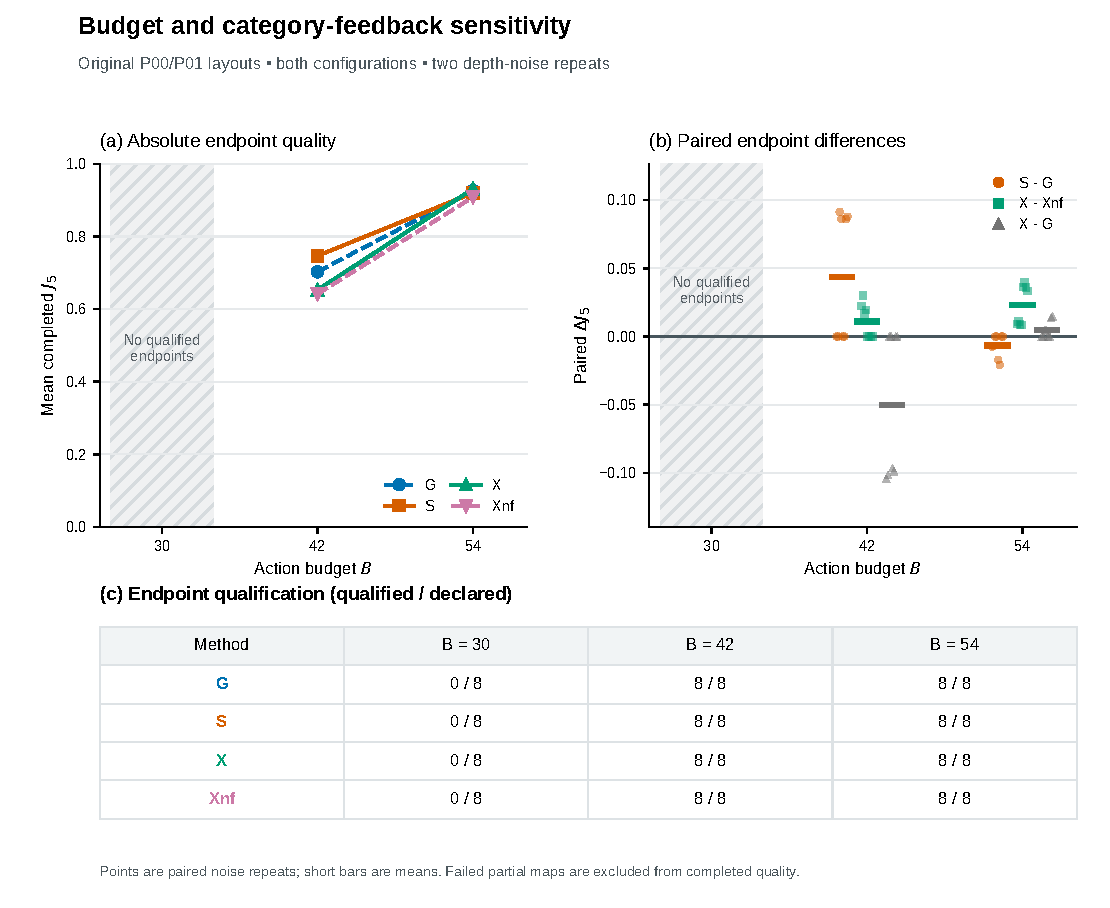
\includegraphics[width=\linewidth,height=.67\textheight,keepaspectratio]{Fig7.pdf}
\caption{Original-layout budget sensitivity. All matched contrasts and qualification counts are retained; budget 30 has no qualified endpoint mean. Short bars indicate complete-pair means rather than confidence intervals across independent scenes}\label{fig:7}
\end{figure}

\hypertarget{transfer-to-changed-background-layouts}{%
\subsection{Transfer to changed background layouts}\label{transfer-to-changed-background-layouts}}

A final protocol fixes two additional layouts before observing results: a side column removes one right-aisle navigation center, while a rear partition interrupts direct rear passage. Both retain the P00 facility family and public templates. The controller, category mapping, sensor noise rule, fusion, evaluation region, 18-action common prefix, and 42-action budget remain unchanged. All legal safe-grid centers are retained; each new layout has 23 centers and 92 oriented poses. The noise seed is the original confirmation seed, so this test adds two background-layout units, not new noise replicates or unseen facility categories. Each layout uses both configurations and G/S, giving eight tasks and four pairs.

All eight tasks complete 42 paid actions and 43 acquired frames, avoid collision, and return to the full initial pose. Table 5 reports every paired endpoint. Mean coverage is identical at 0.934732; mean precision increases from 0.864441 to 0.870224, recall from 0.672455 to 0.704742, and surface F1 from 0.754450 to 0.777445. Mean joint quality increases from 0.705188 to 0.726215, or \textbf{2.9818\%}. The gain is concentrated in the rear-partition h1 condition; the other three conditions retain the same trajectories and endpoint quality. Relative differences at 2 and 10 cm are 2.8176\% and 3.1200\%. These are descriptive paired results from two new layouts; configurations do not increase the number of independent layout units.

\begin{table}[!htbp]
\caption{Changed-background results at 5 cm for all four paired conditions. Coverage is equal within each pair; all eight tasks qualify}\label{tab:5}
\small\setlength{\tabcolsep}{3pt}
\setlength{\JournalTableWidth}{\dimexpr\linewidth-10\tabcolsep\relax}
\begin{tabular}{@{}>{\raggedright\arraybackslash}p{0.26\JournalTableWidth} >{\raggedright\arraybackslash}p{0.148\JournalTableWidth} >{\raggedright\arraybackslash}p{0.148\JournalTableWidth} >{\raggedright\arraybackslash}p{0.148\JournalTableWidth} >{\raggedright\arraybackslash}p{0.148\JournalTableWidth} >{\raggedright\arraybackslash}p{0.148\JournalTableWidth}@{}}
\toprule
Layout / config. & Coverage & G F1 & S F1 & G joint & S joint \\
\midrule
Side column / h0 & 0.954145 & 0.806490 & 0.806490 & 0.769508 & 0.769508 \\
Side column / h1 & 0.955908 & 0.702575 & 0.702575 & 0.671597 & 0.671597 \\
Rear partition / h0 & 0.914439 & 0.806490 & 0.806490 & 0.737485 & 0.737485 \\
Rear partition / h1 & 0.914439 & 0.702246 & 0.794224 & 0.642160 & 0.726269 \\
Mean & 0.934732 & 0.754450 & 0.777445 & 0.705188 & 0.726215 \\
\bottomrule
\end{tabular}
\end{table}

The trajectories in Figure 8 explain the effect's dependence on the available observation routes. In the side-column layout, both initial directions are return-feasible. Category information changes their predicted values but preserves their ordering, so both planners select the same route. In the rear-partition h1 condition, G assigns nearly equal values to the two directions and selects left through its fixed tie rule, whereas S selects right. Up to step 18 their acquired nonsemantic histories and geometric support are identical. The category-conditioned decision changes action 19 and improves endpoint surface recall from 0.595795 to 0.724945. In this condition, \(J_5\) rises from 0.642160 to 0.726269, a relative improvement of \textbf{13.10\%}, at unchanged coverage and action count. This is a complete-route effect: the subsequent measurements differ, so the endpoint gain is not attributed to a single frame.

\begin{figure}[!htbp]
\centering
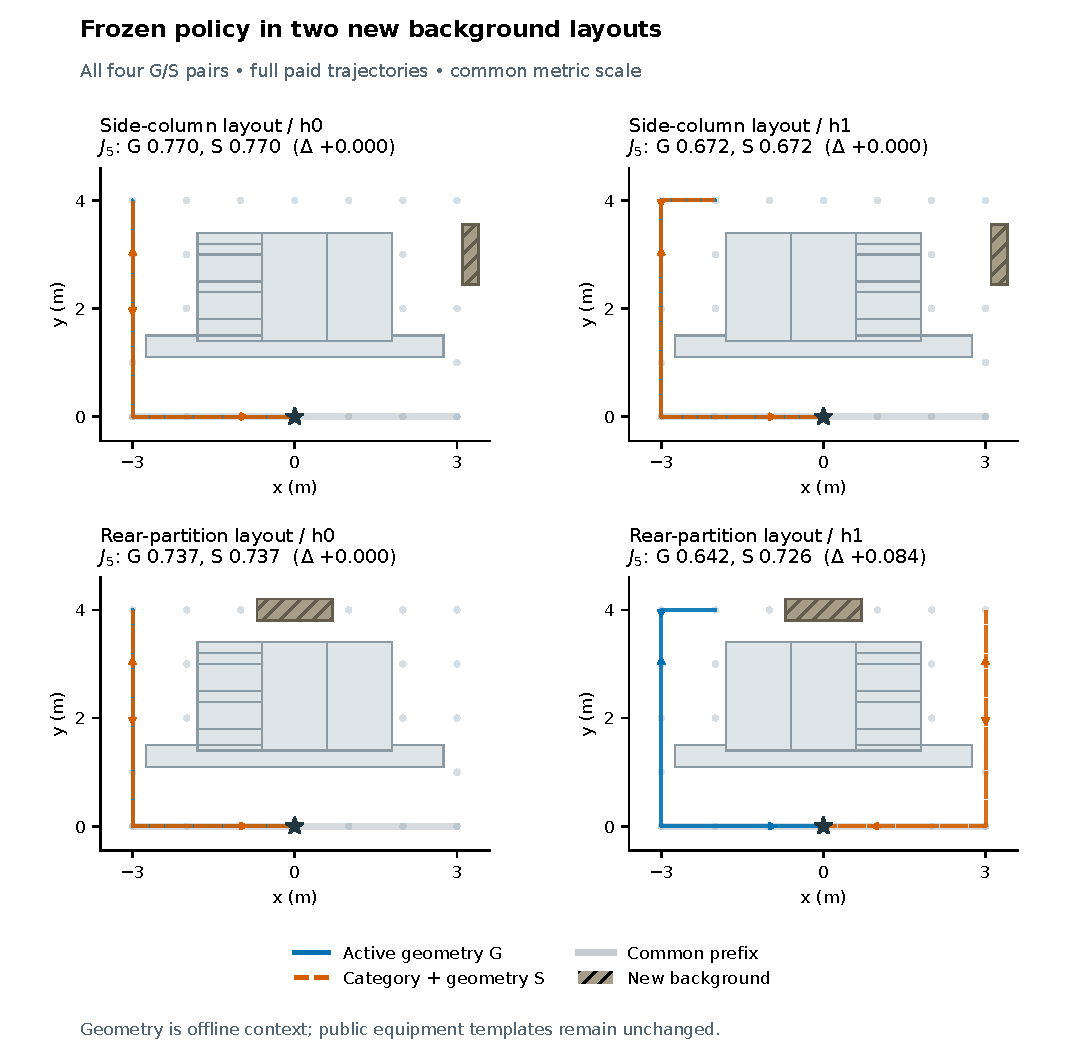
\includegraphics[width=\linewidth,height=.67\textheight,keepaspectratio]{Fig8.pdf}
\caption{Complete paths of all four new background-layout pairs, with recorded headings and a common metric scale. Gray marks the shared paid prefix; hatched regions show added background structures outside the unchanged facility evaluation region. Geometry supplies offline context. Three pairs coincide, while rear-partition h1 diverges at action 19. The companion evidence includes all eight actual endpoint meshes and quality components}\label{fig:8}
\end{figure}

G/S mean travel is 27.0/26.5 m, with 15.0/15.5 turns. Single-thread planning wall time averages 0.0474/0.0484 s per task on an Intel Xeon processor (Sapphire Rapids); complete task times, including sensing, fusion and evaluation, range from 5.0 to 5.8 s. Timing is descriptive for this four-logical-CPU host, not a real-time or cross-hardware benchmark. The controller and all evaluation settings remain fixed throughout this background-layout comparison.

\hypertarget{discussion}{%
\section{Discussion}\label{discussion}}

\hypertarget{when-category-information-has-decision-value}{%
\subsection{When category information has decision value}\label{when-category-information-has-decision-value}}

The results connect three events: an early category cue changes a feasible observation direction, the resulting route acquires different surfaces, and those measurements improve reconstructed surface recall at matched coverage. This chain is visible in both reference h1 configurations and in the rear-partition h1 condition. When category information changes scores without changing their ordering, as in the side-column layout, the resulting trajectory and quality remain unchanged. These cases explain why semantic availability alone is insufficient: the cue must alter an executable decision with a useful downstream consequence.

Budget determines the opportunity for that consequence. At 42 actions, the original and same-family geometry groups show positive mean gains. At 30 actions, the planner cannot meet its predicted coverage and return constraints. At 54 actions, both policies reach complete planar coverage, while S has slightly lower surface precision and joint quality. The decision analysis assumes meaningful directional utilities; the implemented template-exposure surrogate does not model all depth-fusion errors. Its mismatch with measured surface quality is therefore a concrete target for improvement, without treating the observed reversal as evidence for a particular unmeasured sensor-error cause.

\hypertarget{scope-of-the-evidence-and-extensions}{%
\subsection{Scope of the evidence and extensions}\label{scope-of-the-evidence-and-extensions}}

The local method uses public configuration templates, a supplied safe graph, exact poses, and synthetic category cues. These assumptions isolate the planning value of category information but leave natural recognition and estimated-pose SLAM for subsequent validation. The background test adds two layouts within the P00 facility family. Configuration pairs, noise repeats, and reconstruction checkpoints do not constitute additional independent layout samples. The results are descriptive evidence of the tested mechanism, rather than a statistical claim of general superiority. SWAP-I and VISTA-I adapt selected mechanisms to a common CPU setting; the TARE runs demonstrate integration feasibility. These comparisons do not rank the corresponding complete original systems.

A separate multi-facility study explores a different question: whether evidence from one instance improves observation of another instance of the same category. Across 36 runs covering three development layouts and three controller versions, shared and fixed category priors produce identical actions and quality in all nine matched comparisons. Thirty-five runs complete the original evaluation pipeline; the remaining run completes navigation but requires a separately reported numerical evaluation correction. Because this study uses observation macros and a different joint metric, its scores are not pooled with the local results. The complete version-specific tables and the earlier six-parent sharing study, which also did not establish a sharing gain, remain in the companion evidence manuscript. Additional cross-instance semantic benefit is therefore an open extension, separate from the local directional mechanism demonstrated here.

The available ROS 1 robot provides a future implementation platform; the reported performance evidence is entirely simulated. Industrial relevance currently concerns observation after workspace reconfiguration with a static environment during acquisition. Continuous map maintenance and dynamic obstacle avoidance are outside this evaluation.

\hypertarget{conclusion}{%
\section{Conclusion}\label{conclusion}}

This paper presented a category-conditioned observation method combining geometric correction, diagnostic lookahead, and budget-aware execution for facility reconstruction. Category information improves mean joint coverage--surface quality by \textbf{6.16\%} on the reference layouts and \textbf{2.98\%} on two additional background layouts, with unchanged mean coverage in each comparison. Recorded trajectories show that the benefit arises when early category support changes the viewing direction; acquired geometry can also redirect a route after a misleading cue. Budget sensitivity identifies the regime in which this allocation is useful and the limitations of the current exposure surrogate. These findings support category-informed, budget-constrained facility observation and motivate closer alignment between predicted observation value and measured reconstruction quality.

\hypertarget{reproducibility-and-data}{%
\section{Reproducibility and Data}\label{reproducibility-and-data}}

The complete evidence manuscript (Online Resource 4) retains all local and scene-level results, including unchanged outcomes, planning failures, and adverse differences. The supplementary methods (Online Resource 5) describe the separate multi-instance implementation. Archived code, inputs, sensor observations, trajectories, actual meshes, and plotting sources support reproduction. The 128-trial extension, 36 scene-level attempts, and eight background-layout tasks are retained as distinct experiment groups. A representative 43-frame saved replay reproduces controller outputs and reconstructed meshes exactly; intermediate reconstruction checkpoints reuse existing observations.

\begin{thebibliography}{99}
\bibitem{ref9} World Economic Forum. Physical AI: Powering the New Age of Industrial Operations. White paper, 2025-09-04. \href{https://www.weforum.org/publications/physical-ai-powering-the-new-age-of-industrial-operations/}{Official white paper}.

\bibitem{ref10} Placed J. A., Strader J., Carrillo H., Atanasov N., Indelman V., Carlone L., Castellanos J. A. A Survey on Active Simultaneous Localization and Mapping: State of the Art and New Frontiers. IEEE Transactions on Robotics, 2023. \url{https://doi.org/10.1109/TRO.2023.3248510}.

\bibitem{ref5} Cao C., Zhu H., Choset H., Zhang J. TARE: A Hierarchical Framework for Efficiently Exploring Complex 3D Environments. RSS, 2021. \url{https://doi.org/10.15607/RSS.2021.XVII.018}.

\bibitem{ref1} Chaplot D. S., Gandhi D., Gupta S., Gupta A., Salakhutdinov R. Learning to Explore using Active Neural SLAM. ICLR, 2020. Author manuscript: \url{https://doi.org/10.48550/arXiv.2004.05155}.

\bibitem{ref6} Chen X., Li Q., Wang T., Xue T., Pang J. GenNBV: Generalizable Next-Best-View Policy for Active 3D Reconstruction. CVPR, 2024:16436--16445. \url{https://doi.org/10.1109/CVPR52733.2024.01555}.

\bibitem{ref4} Zhou Q.-Y., Park J., Koltun V. Open3D: A Modern Library for 3D Data Processing. arXiv:1801.09847, 2018. \url{https://doi.org/10.48550/arXiv.1801.09847}.

\bibitem{ref11} Curless B., Levoy M. A Volumetric Method for Building Complex Models from Range Images. Proceedings of SIGGRAPH, 1996:303--312. \url{https://doi.org/10.1145/237170.237269}.

\bibitem{ref2} Dharmadhikari M., Alexis K. Semantics-aware Exploration and Inspection Path Planning. ICRA, 2023. \url{https://doi.org/10.1109/ICRA48891.2023.10160469}.

\bibitem{ref7} Dharmadhikari M., Alexis K. Semantics-Aware Predictive Inspection Path Planning. IEEE Transactions on Field Robotics, 2025. \url{https://doi.org/10.1109/TFR.2025.3578402}.

\bibitem{ref3} Nagami K., Chen T., Yu J., Shorinwa O., Adang M., Dougherty C., Cristofalo E., Schwager M. VISTA: Open-Vocabulary, Task-Relevant Robot Exploration With Online Semantic Gaussian Splatting. IEEE Robotics and Automation Letters, 11(3):3150--3157, 2026. \url{https://doi.org/10.1109/LRA.2026.3653276}.

\bibitem{ref8} Chen L., Zhan H., Yin H., Xu Y., Mordohai P. Understanding while Exploring: Semantics-driven Active Mapping. Advances in Neural Information Processing Systems, 38, 2025. \url{https://doi.org/10.52202/085713-1113}.

\bibitem{ref12} Kaelbling L. P., Littman M. L., Cassandra A. R. Planning and Acting in Partially Observable Stochastic Domains. Artificial Intelligence, 101(1--2):99--134, 1998. \url{https://doi.org/10.1016/S0004-3702(98)00023-X}.

\bibitem{ref13} Hollinger G. A., Sukhatme G. S. Sampling-based Robotic Information Gathering Algorithms. The International Journal of Robotics Research, 33(9):1271--1287, 2014. \url{https://doi.org/10.1177/0278364914533443}.

\bibitem{ref14} Knapitsch A., Park J., Zhou Q.-Y., Koltun V. Tanks and Temples: Benchmarking Large-Scale Scene Reconstruction. ACM Transactions on Graphics, 36(4), 2017. \url{https://doi.org/10.1145/3072959.3073599}.
\end{thebibliography}

\section*{Statements and Declarations}
\subsection*{Funding}
\textit{Author confirmation required:} \underline{\hspace{5cm}}
\subsection*{Competing interests}
\textit{Author confirmation required:} \underline{\hspace{5cm}}
\subsection*{Author contributions}
\textit{Author confirmation required:} \underline{\hspace{5cm}}
\subsection*{Data and code availability}
See the Reproducibility and Data section and the accompanying Online Resources.
The final public version identifier and any access restrictions require author confirmation.
\subsection*{AI assistance disclosure: draft for author confirmation}
OpenAI Codex assisted with manuscript organization and revision and with developing
experiment, analysis, and plotting code. Tool/model versions, the extent of assistance,
and the authors' verification and responsibility statement must be completed before submission.
This draft disclosure does not assert that the authors have already approved the manuscript.

\subsection*{Online Resources}
Online Resource 1: matched detail views (\texttt{ESM\_1.pdf}).

Online Resource 2: Complete precision/recall figure (\texttt{ESM\_2.pdf}).

Online Resource 3: actual stage meshes (\texttt{ESM\_3.pdf}).

Online Resource 4: complete evidence manuscript (\texttt{ESM\_4.pdf}).

Online Resource 5: supplementary methods (\texttt{ESM\_5.pdf}).
\end{document}
